% Options for packages loaded elsewhere
\PassOptionsToPackage{unicode}{hyperref}
\PassOptionsToPackage{hyphens}{url}
\PassOptionsToPackage{dvipsnames,svgnames,x11names}{xcolor}
%
\documentclass[
  ignorenonframetext,
]{beamer}
\usepackage{pgfpages}
\setbeamertemplate{caption}[numbered]
\setbeamertemplate{caption label separator}{: }
\setbeamercolor{caption name}{fg=normal text.fg}
\beamertemplatenavigationsymbolsempty
% Prevent slide breaks in the middle of a paragraph
\widowpenalties 1 10000
\raggedbottom

\usepackage{amsmath,amssymb}
\usepackage{iftex}
\ifPDFTeX
  \usepackage[T1]{fontenc}
  \usepackage[utf8]{inputenc}
  \usepackage{textcomp} % provide euro and other symbols
\else % if luatex or xetex
  \usepackage{unicode-math}
  \defaultfontfeatures{Scale=MatchLowercase}
  \defaultfontfeatures[\rmfamily]{Ligatures=TeX,Scale=1}
\fi
\usepackage{lmodern}
\usetheme[]{AnnArbor}
\usecolortheme{dolphin}
\usefonttheme{structurebold}
\ifPDFTeX\else  
    % xetex/luatex font selection
\fi
% Use upquote if available, for straight quotes in verbatim environments
\IfFileExists{upquote.sty}{\usepackage{upquote}}{}
\IfFileExists{microtype.sty}{% use microtype if available
  \usepackage[]{microtype}
  \UseMicrotypeSet[protrusion]{basicmath} % disable protrusion for tt fonts
}{}
\makeatletter
\@ifundefined{KOMAClassName}{% if non-KOMA class
  \IfFileExists{parskip.sty}{%
    \usepackage{parskip}
  }{% else
    \setlength{\parindent}{0pt}
    \setlength{\parskip}{6pt plus 2pt minus 1pt}}
}{% if KOMA class
  \KOMAoptions{parskip=half}}
\makeatother
\usepackage{xcolor}
\newif\ifbibliography
\setlength{\emergencystretch}{3em} % prevent overfull lines
\setcounter{secnumdepth}{-\maxdimen} % remove section numbering

\usepackage{color}
\usepackage{fancyvrb}
\newcommand{\VerbBar}{|}
\newcommand{\VERB}{\Verb[commandchars=\\\{\}]}
\DefineVerbatimEnvironment{Highlighting}{Verbatim}{commandchars=\\\{\}}
% Add ',fontsize=\small' for more characters per line
\usepackage{framed}
\definecolor{shadecolor}{RGB}{241,243,245}
\newenvironment{Shaded}{\begin{snugshade}}{\end{snugshade}}
\newcommand{\AlertTok}[1]{\textcolor[rgb]{0.68,0.00,0.00}{#1}}
\newcommand{\AnnotationTok}[1]{\textcolor[rgb]{0.37,0.37,0.37}{#1}}
\newcommand{\AttributeTok}[1]{\textcolor[rgb]{0.40,0.45,0.13}{#1}}
\newcommand{\BaseNTok}[1]{\textcolor[rgb]{0.68,0.00,0.00}{#1}}
\newcommand{\BuiltInTok}[1]{\textcolor[rgb]{0.00,0.23,0.31}{#1}}
\newcommand{\CharTok}[1]{\textcolor[rgb]{0.13,0.47,0.30}{#1}}
\newcommand{\CommentTok}[1]{\textcolor[rgb]{0.37,0.37,0.37}{#1}}
\newcommand{\CommentVarTok}[1]{\textcolor[rgb]{0.37,0.37,0.37}{\textit{#1}}}
\newcommand{\ConstantTok}[1]{\textcolor[rgb]{0.56,0.35,0.01}{#1}}
\newcommand{\ControlFlowTok}[1]{\textcolor[rgb]{0.00,0.23,0.31}{\textbf{#1}}}
\newcommand{\DataTypeTok}[1]{\textcolor[rgb]{0.68,0.00,0.00}{#1}}
\newcommand{\DecValTok}[1]{\textcolor[rgb]{0.68,0.00,0.00}{#1}}
\newcommand{\DocumentationTok}[1]{\textcolor[rgb]{0.37,0.37,0.37}{\textit{#1}}}
\newcommand{\ErrorTok}[1]{\textcolor[rgb]{0.68,0.00,0.00}{#1}}
\newcommand{\ExtensionTok}[1]{\textcolor[rgb]{0.00,0.23,0.31}{#1}}
\newcommand{\FloatTok}[1]{\textcolor[rgb]{0.68,0.00,0.00}{#1}}
\newcommand{\FunctionTok}[1]{\textcolor[rgb]{0.28,0.35,0.67}{#1}}
\newcommand{\ImportTok}[1]{\textcolor[rgb]{0.00,0.46,0.62}{#1}}
\newcommand{\InformationTok}[1]{\textcolor[rgb]{0.37,0.37,0.37}{#1}}
\newcommand{\KeywordTok}[1]{\textcolor[rgb]{0.00,0.23,0.31}{\textbf{#1}}}
\newcommand{\NormalTok}[1]{\textcolor[rgb]{0.00,0.23,0.31}{#1}}
\newcommand{\OperatorTok}[1]{\textcolor[rgb]{0.37,0.37,0.37}{#1}}
\newcommand{\OtherTok}[1]{\textcolor[rgb]{0.00,0.23,0.31}{#1}}
\newcommand{\PreprocessorTok}[1]{\textcolor[rgb]{0.68,0.00,0.00}{#1}}
\newcommand{\RegionMarkerTok}[1]{\textcolor[rgb]{0.00,0.23,0.31}{#1}}
\newcommand{\SpecialCharTok}[1]{\textcolor[rgb]{0.37,0.37,0.37}{#1}}
\newcommand{\SpecialStringTok}[1]{\textcolor[rgb]{0.13,0.47,0.30}{#1}}
\newcommand{\StringTok}[1]{\textcolor[rgb]{0.13,0.47,0.30}{#1}}
\newcommand{\VariableTok}[1]{\textcolor[rgb]{0.07,0.07,0.07}{#1}}
\newcommand{\VerbatimStringTok}[1]{\textcolor[rgb]{0.13,0.47,0.30}{#1}}
\newcommand{\WarningTok}[1]{\textcolor[rgb]{0.37,0.37,0.37}{\textit{#1}}}

\providecommand{\tightlist}{%
  \setlength{\itemsep}{0pt}\setlength{\parskip}{0pt}}\usepackage{longtable,booktabs,array}
\usepackage{calc} % for calculating minipage widths
\usepackage{caption}
% Make caption package work with longtable
\makeatletter
\def\fnum@table{\tablename~\thetable}
\makeatother
\usepackage{graphicx}
\makeatletter
\def\maxwidth{\ifdim\Gin@nat@width>\linewidth\linewidth\else\Gin@nat@width\fi}
\def\maxheight{\ifdim\Gin@nat@height>\textheight\textheight\else\Gin@nat@height\fi}
\makeatother
% Scale images if necessary, so that they will not overflow the page
% margins by default, and it is still possible to overwrite the defaults
% using explicit options in \includegraphics[width, height, ...]{}
\setkeys{Gin}{width=\maxwidth,height=\maxheight,keepaspectratio}
% Set default figure placement to htbp
\makeatletter
\def\fps@figure{htbp}
\makeatother
% definitions for citeproc citations
\NewDocumentCommand\citeproctext{}{}
\NewDocumentCommand\citeproc{mm}{%
  \begingroup\def\citeproctext{#2}\cite{#1}\endgroup}
\makeatletter
 % allow citations to break across lines
 \let\@cite@ofmt\@firstofone
 % avoid brackets around text for \cite:
 \def\@biblabel#1{}
 \def\@cite#1#2{{#1\if@tempswa , #2\fi}}
\makeatother
\newlength{\cslhangindent}
\setlength{\cslhangindent}{1.5em}
\newlength{\csllabelwidth}
\setlength{\csllabelwidth}{3em}
\newenvironment{CSLReferences}[2] % #1 hanging-indent, #2 entry-spacing
 {\begin{list}{}{%
  \setlength{\itemindent}{0pt}
  \setlength{\leftmargin}{0pt}
  \setlength{\parsep}{0pt}
  % turn on hanging indent if param 1 is 1
  \ifodd #1
   \setlength{\leftmargin}{\cslhangindent}
   \setlength{\itemindent}{-1\cslhangindent}
  \fi
  % set entry spacing
  \setlength{\itemsep}{#2\baselineskip}}}
 {\end{list}}
\usepackage{calc}
\newcommand{\CSLBlock}[1]{\hfill\break\parbox[t]{\linewidth}{\strut\ignorespaces#1\strut}}
\newcommand{\CSLLeftMargin}[1]{\parbox[t]{\csllabelwidth}{\strut#1\strut}}
\newcommand{\CSLRightInline}[1]{\parbox[t]{\linewidth - \csllabelwidth}{\strut#1\strut}}
\newcommand{\CSLIndent}[1]{\hspace{\cslhangindent}#1}

\usepackage{booktabs}
\usepackage{longtable}
\usepackage{array}
\usepackage{multirow}
\usepackage{wrapfig}
\usepackage{float}
\usepackage{colortbl}
\usepackage{pdflscape}
\usepackage{tabu}
\usepackage{threeparttable}
\usepackage{threeparttablex}
\usepackage[normalem]{ulem}
\usepackage{makecell}
\usepackage{xcolor}

% logo
\titlegraphic{
\includegraphics[width=4cm]{../000_logos/logo-blue-vertical}}
\logo{\ifnum\thepage>1
\includegraphics[width=0.5cm]{../000_logos/logo-blue-vertical}\fi}

% UMNG: Manual de image institucional

% Colors

% Umng
\definecolor{yellow}{HTML}{fdc600}
\definecolor{red}{HTML}{ee2a24}

% Estudios a Distancia
\definecolor{blue1}{HTML}{12245b}
\definecolor{blue2}{HTML}{767ca6}
\definecolor{blue3}{HTML}{cad2ec}

% Modify items
\setbeamercolor{palette primary}{bg=blue3}
\setbeamercolor{palette tertiary}{bg=blue1}
\setbeamercolor{frametitle}{bg=yellow}

% Hyperlinks
\hypersetup{
  linkcolor=red,
  citecolor=red
}

\makeatletter
\@ifpackageloaded{caption}{}{\usepackage{caption}}
\AtBeginDocument{%
\ifdefined\contentsname
  \renewcommand*\contentsname{Table of contents}
\else
  \newcommand\contentsname{Table of contents}
\fi
\ifdefined\listfigurename
  \renewcommand*\listfigurename{List of Figures}
\else
  \newcommand\listfigurename{List of Figures}
\fi
\ifdefined\listtablename
  \renewcommand*\listtablename{List of Tables}
\else
  \newcommand\listtablename{List of Tables}
\fi
\ifdefined\figurename
  \renewcommand*\figurename{Figure}
\else
  \newcommand\figurename{Figure}
\fi
\ifdefined\tablename
  \renewcommand*\tablename{Table}
\else
  \newcommand\tablename{Table}
\fi
}
\@ifpackageloaded{float}{}{\usepackage{float}}
\floatstyle{ruled}
\@ifundefined{c@chapter}{\newfloat{codelisting}{h}{lop}}{\newfloat{codelisting}{h}{lop}[chapter]}
\floatname{codelisting}{Listing}
\newcommand*\listoflistings{\listof{codelisting}{List of Listings}}
\makeatother
\makeatletter
\makeatother
\makeatletter
\@ifpackageloaded{caption}{}{\usepackage{caption}}
\@ifpackageloaded{subcaption}{}{\usepackage{subcaption}}
\makeatother

\ifLuaTeX
\usepackage[bidi=basic]{babel}
\else
\usepackage[bidi=default]{babel}
\fi
\babelprovide[main,import]{english}
% get rid of language-specific shorthands (see #6817):
\let\LanguageShortHands\languageshorthands
\def\languageshorthands#1{}
\ifLuaTeX
  \usepackage{selnolig}  % disable illegal ligatures
\fi
\usepackage{bookmark}

\IfFileExists{xurl.sty}{\usepackage{xurl}}{} % add URL line breaks if available
\urlstyle{same} % disable monospaced font for URLs
\hypersetup{
  pdftitle={Business Case},
  pdfauthor={Luis Francisco Gómez López},
  pdflang={en},
  colorlinks=true,
  linkcolor={Maroon},
  filecolor={Maroon},
  citecolor={Blue},
  urlcolor={Blue},
  pdfcreator={LaTeX via pandoc}}


\title{Business Case}
\author{Luis Francisco Gómez López}
\date{2024-08-01}
\institute{FAEDIS}

\begin{document}
\frame{\titlepage}

\renewcommand*\contentsname{Table of contents}
\begin{frame}[allowframebreaks]
  \frametitle{Table of contents}
  \tableofcontents[hideallsubsections]
\end{frame}

\section{Please Read Me}\label{please-read-me}

\begin{frame}{}
\phantomsection\label{section}
\begin{itemize}
\tightlist
\item
  This presentation is based on a business case taken from the course
  \href{https://university.business-science.io/p/ds4b-101-r-business-analysis-r}{Data
  Science for Business Part 1} offered by the company
  \href{https://www.business-science.io/}{Business Science} and adapted
  to be in line with the topics covered in
  (\citeproc{ref-chapman_r_2019}{Chapman and Feit 2019})
\end{itemize}
\end{frame}

\section{Purpose}\label{purpose}

\begin{frame}{}
\phantomsection\label{section-1}
\begin{itemize}
\tightlist
\item
  Deliver essential knowledge within a minimal timeframe by employing
  hands-on learning techniques to enhance productivity in the R
  programming language
\end{itemize}
\end{frame}

\section{Business Case}\label{business-case}

\begin{frame}{}
\phantomsection\label{section-2}
\begin{itemize}
\item
  You and your team will work for a corporation located in Wilton,
  Connecticut, United States that supplies bicycle frames and other
  components related to bicycles to different bicycle shops through the
  United States.
\item
  Your team is assigned to complete 2 tasks:

  \begin{itemize}
  \item
    Support the Research and Development (R \& D) division in
    identifying potential new products and pricing them by using data
    collected from the bicycle shops.
  \item
    Support the marketing team in the creation of a marketing
    segmentation clustering model by using data collected from to the
    bicycle shops to offer more personalized products and messaging
    them.
  \end{itemize}
\end{itemize}
\end{frame}

\begin{frame}{}
\phantomsection\label{section-3}
\begin{itemize}
\item
  Business unit: Cannondale Bicycle Corporation (Manufacturer)

  \begin{itemize}
  \item
    Location: USA
  \item
    Product: Bicycle frames
  \item
    Retailers: Bikeshops located through USA

    \begin{itemize}
    \tightlist
    \item
      We are not going to analyze the business-to-customer (B2B)
      subchannel (Retailer to Customer) where the focus will be on the
      business-to-business (B2B) subchannel (Manufacturer to Retailer)
    \end{itemize}
  \end{itemize}
\end{itemize}

\begin{figure}

\centering{

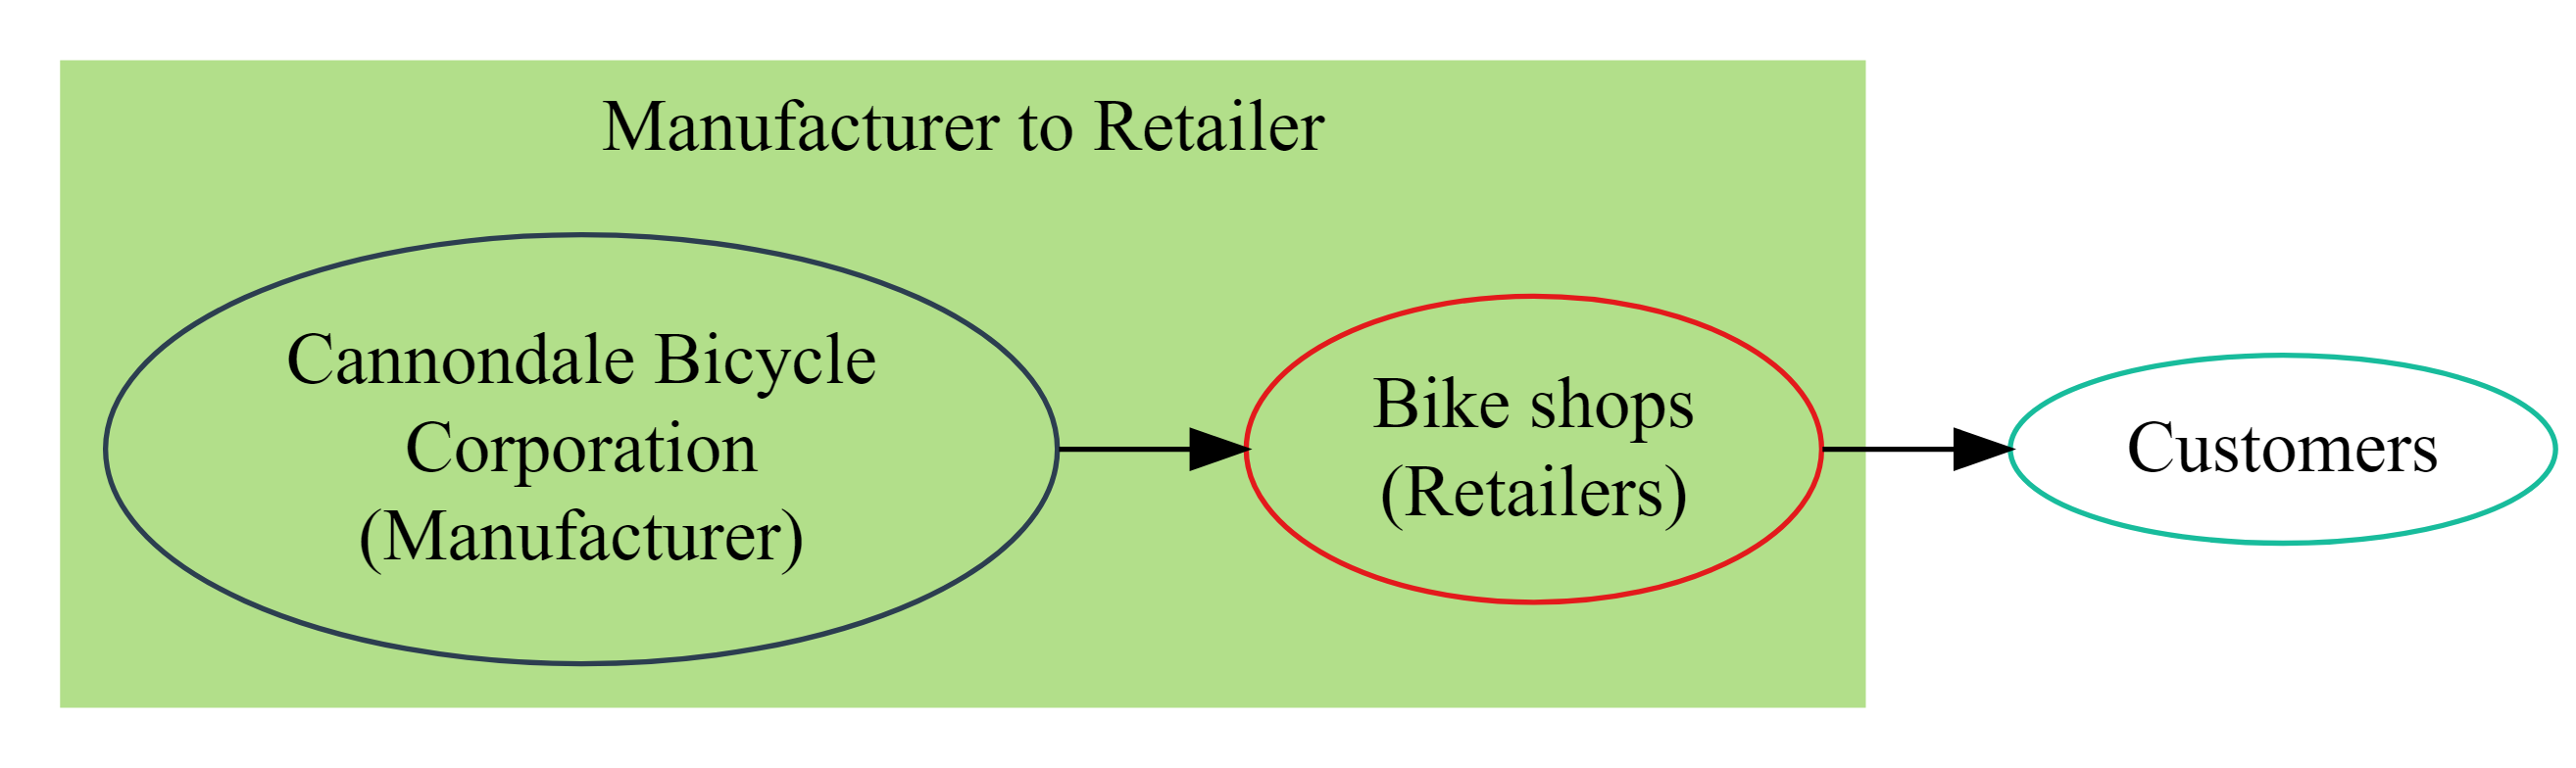
\includegraphics[width=4in,height=2in]{001_b_business_case_files/figure-beamer/dot-figure-1.png}

}

\caption{\label{fig-distribution-channel}Distribution channel}

\end{figure}%
\end{frame}

\begin{frame}{}
\phantomsection\label{section-4}
\tiny

\begin{figure}

\centering{

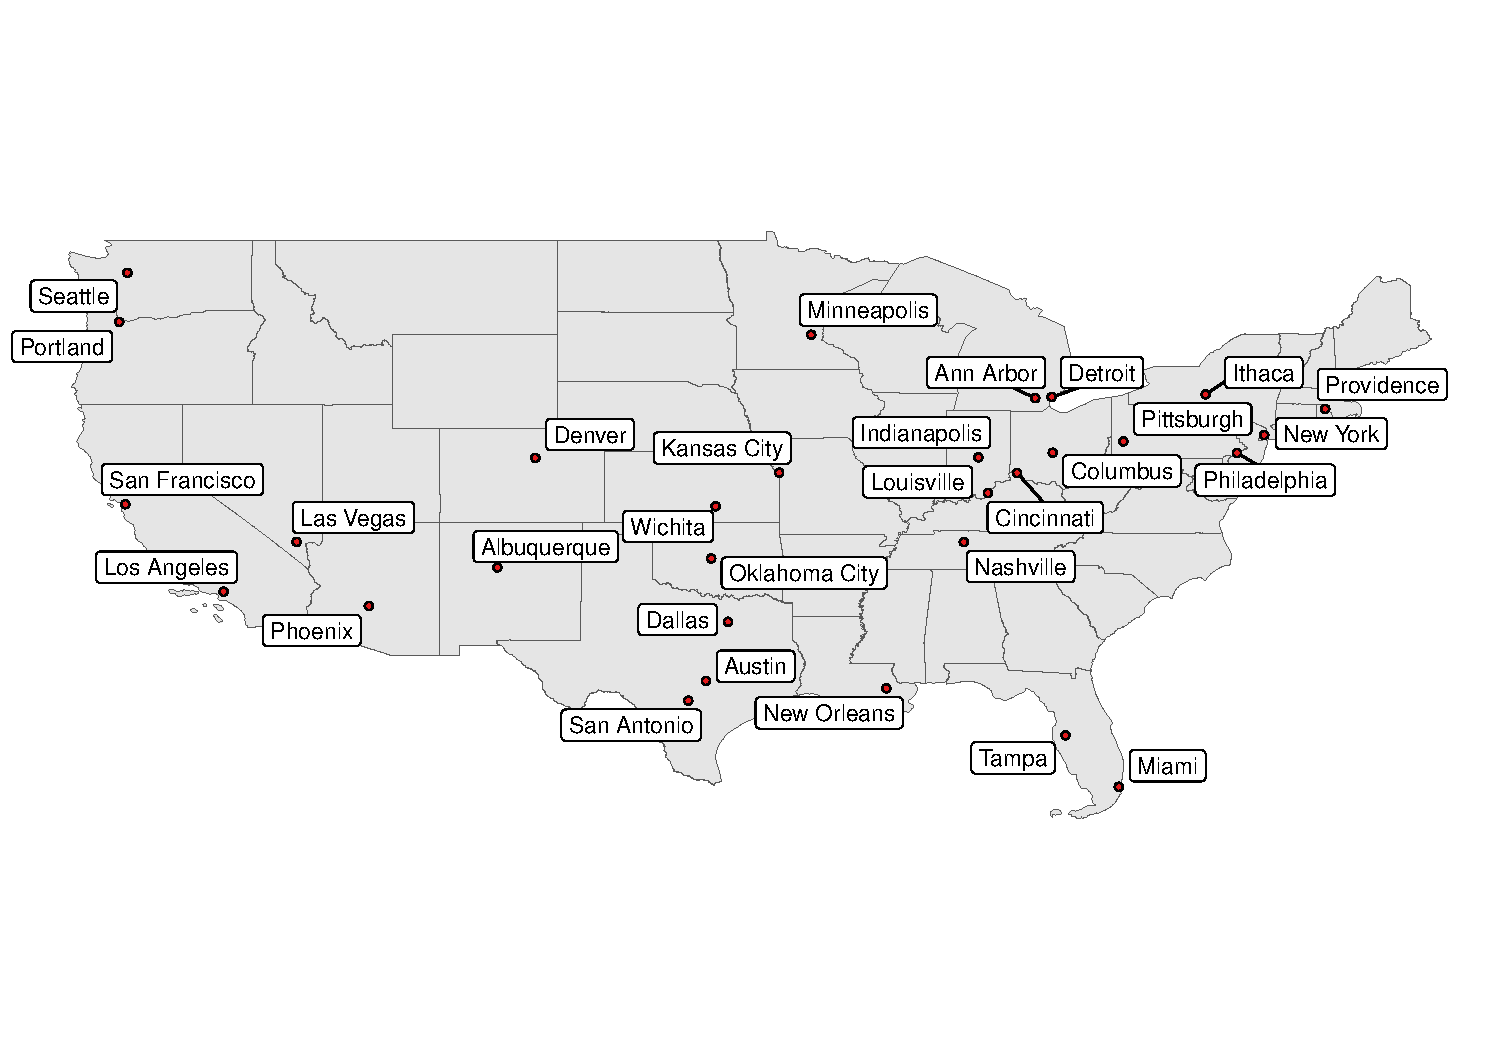
\includegraphics[width=0.85\textwidth,height=\textheight]{001_b_business_case_files/figure-beamer/fig-bike-shops-locations-1.pdf}

}

\caption{\label{fig-bike-shops-locations}Bike shops locations}

\end{figure}%
\end{frame}

\begin{frame}{}
\phantomsection\label{section-5}
\begin{figure}[H]

{\centering 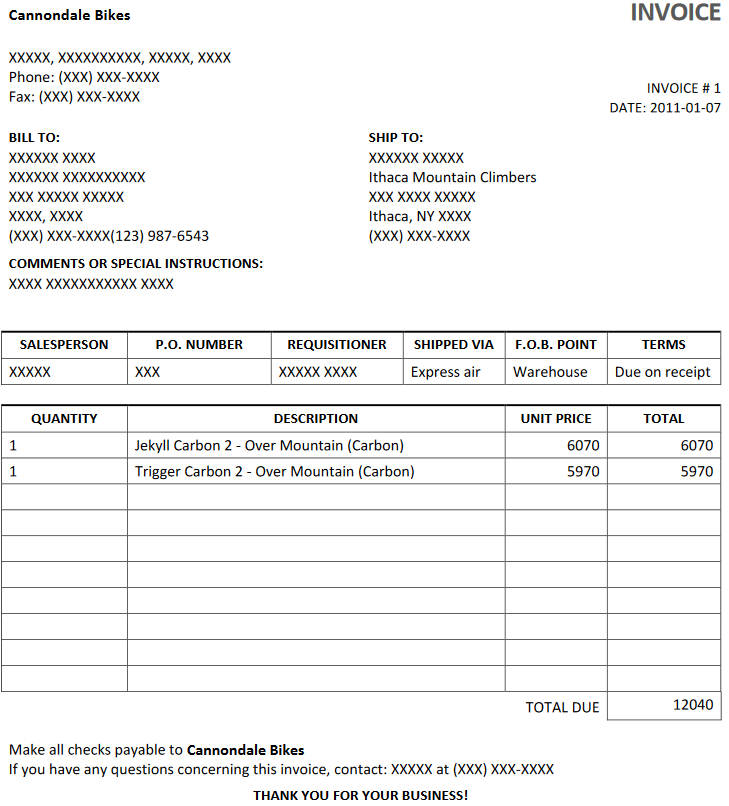
\includegraphics[width=3.64583in,height=2.96875in]{../000_images/001_example_invoice_transaction.png}

}

\caption{Invoice example representing a transaction}

\end{figure}%
\end{frame}

\begin{frame}{}
\phantomsection\label{section-6}
\begin{itemize}
\item
  Entities

  \begin{itemize}
  \item
    \textbf{Product}

    \begin{itemize}
    \tightlist
    \item
      Product Id: unique product identification number
    \item
      Model: model name of the bicycle
    \item
      Category primary: main bicycle category (Mountain, Road)
    \item
      Category secondary: More specific bicycle category (9 categories)
    \item
      Frame: bicycle frame material (Carbon, Aluminum)
    \end{itemize}
  \item
    \textbf{Retailer}

    \begin{itemize}
    \tightlist
    \item
      Bike shop Id: unique bike shop identification number
    \item
      Bike shop name
    \item
      Bike shop state: state that the bike shop is located
    \item
      Bike shop city: city that the bike shop is located
    \item
      Latitude: geograhpic latitude of the bike shop location
    \item
      Longitude: geograhpic longitude of the bike shop location
    \end{itemize}
  \end{itemize}
\end{itemize}
\end{frame}

\begin{frame}{}
\phantomsection\label{section-7}
\begin{itemize}
\item
  Entities

  \begin{itemize}
  \item
    \textbf{Closed order}

    \begin{itemize}
    \tightlist
    \item
      Order Id: unique order identification number
    \item
      Order date: date the order was placed
    \item
      Order line: sequential identification number for products on an
      order
    \item
      Quantity: number of units purchased by the retailer
    \item
      Price: unit price of the bicycle
    \item
      Bike shop Id: unique bike shop identification number
    \item
      Product Id: unique product identification number
    \end{itemize}
  \end{itemize}
\end{itemize}
\end{frame}

\begin{frame}{}
\phantomsection\label{section-8}
\begin{figure}[H]

{\centering 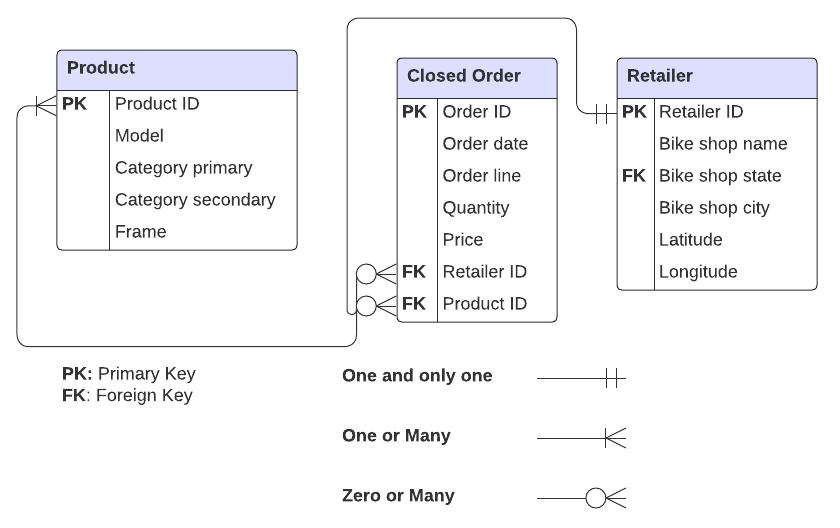
\includegraphics[width=3.64583in,height=3.64583in]{../000_images/001_database_er_diagram_foot_crow_notation.png}

}

\caption{Database Entity Relationship Diagram (ERD)\footnote<.->{See
  (\citeproc{ref-abba_crows_2022}{Abba 2022})}}

\end{figure}%
\end{frame}

\begin{frame}[fragile]{}
\phantomsection\label{section-9}
\begin{itemize}
\tightlist
\item
  Understand the business data
\end{itemize}

\tiny

\begin{Shaded}
\begin{Highlighting}[]
\FunctionTok{library}\NormalTok{(tidyverse) }\CommentTok{\# Remember to load the tidyverse library}
\FunctionTok{library}\NormalTok{(sweep) }\CommentTok{\# Remember to load the sweep library}
\end{Highlighting}
\end{Shaded}

\begin{Shaded}
\begin{Highlighting}[]
\NormalTok{bike\_sales}
\end{Highlighting}
\end{Shaded}

\begin{verbatim}
# A tibble: 15,644 x 17
   order.date order.id order.line quantity price price.ext customer.id
   <date>        <dbl>      <int>    <dbl> <dbl>     <dbl>       <dbl>
 1 2011-01-07        1          1        1  6070      6070           2
 2 2011-01-07        1          2        1  5970      5970           2
 3 2011-01-10        2          1        1  2770      2770          10
 4 2011-01-10        2          2        1  5970      5970          10
 5 2011-01-10        3          1        1 10660     10660           6
 6 2011-01-10        3          2        1  3200      3200           6
 7 2011-01-10        3          3        1 12790     12790           6
 8 2011-01-10        3          4        1  5330      5330           6
 9 2011-01-10        3          5        1  1570      1570           6
10 2011-01-11        4          1        1  4800      4800          22
# i 15,634 more rows
# i 10 more variables: bikeshop.name <chr>, bikeshop.city <chr>,
#   bikeshop.state <chr>, latitude <dbl>, longitude <dbl>, product.id <dbl>,
#   model <chr>, category.primary <chr>, category.secondary <chr>, frame <chr>
\end{verbatim}

\normalsize

\begin{itemize}
\tightlist
\item
  Only works in RStudio IDE
\end{itemize}

\tiny

\begin{Shaded}
\begin{Highlighting}[]
\NormalTok{bike\_sales }\SpecialCharTok{|\textgreater{}} \FunctionTok{View}\NormalTok{()}
\end{Highlighting}
\end{Shaded}
\end{frame}

\begin{frame}{}
\phantomsection\label{section-10}
\begin{itemize}
\item
  Products

  \begin{itemize}
  \tightlist
  \item
    97 bicycle models
  \end{itemize}
\end{itemize}

\begin{table}

\caption{\label{tbl-products-first}First 5 products}

\centering{

\centering\begingroup\fontsize{7}{9}\selectfont

\begin{tabular}{rllll}
\toprule
\textbf{Product Id} & \textbf{Model} & \textbf{Primary category} & \textbf{Secondary category} & \textbf{Frame}\\
\midrule
\cellcolor{gray!10}{48} & \cellcolor{gray!10}{Jekyll Carbon 2} & \cellcolor{gray!10}{Mountain} & \cellcolor{gray!10}{Over Mountain} & \cellcolor{gray!10}{Carbon}\\
52 & Trigger Carbon 2 & Mountain & Over Mountain & Carbon\\
\cellcolor{gray!10}{76} & \cellcolor{gray!10}{Beast of the East 1} & \cellcolor{gray!10}{Mountain} & \cellcolor{gray!10}{Trail} & \cellcolor{gray!10}{Aluminum}\\
2 & Supersix Evo Hi-Mod Team & Road & Elite Road & Carbon\\
\cellcolor{gray!10}{50} & \cellcolor{gray!10}{Jekyll Carbon 4} & \cellcolor{gray!10}{Mountain} & \cellcolor{gray!10}{Over Mountain} & \cellcolor{gray!10}{Carbon}\\
\bottomrule
\end{tabular}
\endgroup{}

}

\end{table}%
\end{frame}

\begin{frame}{}
\phantomsection\label{section-11}
\begin{itemize}
\item
  Retailers

  \begin{itemize}
  \tightlist
  \item
    30 bike shops
  \end{itemize}
\end{itemize}

\begin{table}

\caption{\label{tbl-retailers-first}First 5 retailers}

\centering{

\centering\begingroup\fontsize{7}{9}\selectfont

\begin{tabular}{rlllrr}
\toprule
\textbf{Retailer Id} & \textbf{Bike shop name} & \textbf{City} & \textbf{State} & \textbf{Latitude} & \textbf{Longitude}\\
\midrule
\cellcolor{gray!10}{2} & \cellcolor{gray!10}{Ithaca Mountain Climbers} & \cellcolor{gray!10}{Ithaca} & \cellcolor{gray!10}{NY} & \cellcolor{gray!10}{42.44396} & \cellcolor{gray!10}{-76.50188}\\
10 & Kansas City 29ers & Kansas City & KS & 39.11405 & -94.62746\\
\cellcolor{gray!10}{6} & \cellcolor{gray!10}{Louisville Race Equipment} & \cellcolor{gray!10}{Louisville} & \cellcolor{gray!10}{KY} & \cellcolor{gray!10}{38.25267} & \cellcolor{gray!10}{-85.75846}\\
22 & Ann Arbor Speed & Ann Arbor & MI & 42.28083 & -83.74304\\
\cellcolor{gray!10}{8} & \cellcolor{gray!10}{Denver Bike Shop} & \cellcolor{gray!10}{Denver} & \cellcolor{gray!10}{CO} & \cellcolor{gray!10}{39.73924} & \cellcolor{gray!10}{-104.99025}\\
\bottomrule
\end{tabular}
\endgroup{}

}

\end{table}%
\end{frame}

\begin{frame}{}
\phantomsection\label{section-12}
\begin{itemize}
\item
  Closed orders

  \begin{itemize}
  \tightlist
  \item
    2000 orders
  \end{itemize}
\end{itemize}

\begin{table}

\caption{\label{tbl-transactions-first}First 5 orders}

\centering{

\centering\begingroup\fontsize{7}{9}\selectfont

\begin{tabular}{lrrrrrr}
\toprule
\textbf{Order date} & \textbf{Order Id} & \textbf{Order line} & \textbf{Quantity} & \textbf{Price} & \textbf{Retailer Id} & \textbf{Product Id}\\
\midrule
\cellcolor{gray!10}{2011-01-07} & \cellcolor{gray!10}{1} & \cellcolor{gray!10}{1} & \cellcolor{gray!10}{1} & \cellcolor{gray!10}{6070} & \cellcolor{gray!10}{2} & \cellcolor{gray!10}{48}\\
2011-01-07 & 1 & 2 & 1 & 5970 & 2 & 52\\
\cellcolor{gray!10}{2011-01-10} & \cellcolor{gray!10}{2} & \cellcolor{gray!10}{1} & \cellcolor{gray!10}{1} & \cellcolor{gray!10}{2770} & \cellcolor{gray!10}{10} & \cellcolor{gray!10}{76}\\
2011-01-10 & 2 & 2 & 1 & 5970 & 10 & 52\\
\cellcolor{gray!10}{2011-01-10} & \cellcolor{gray!10}{3} & \cellcolor{gray!10}{1} & \cellcolor{gray!10}{1} & \cellcolor{gray!10}{10660} & \cellcolor{gray!10}{6} & \cellcolor{gray!10}{2}\\
2011-01-10 & 3 & 2 & 1 & 3200 & 6 & 50\\
\cellcolor{gray!10}{2011-01-10} & \cellcolor{gray!10}{3} & \cellcolor{gray!10}{3} & \cellcolor{gray!10}{1} & \cellcolor{gray!10}{12790} & \cellcolor{gray!10}{6} & \cellcolor{gray!10}{1}\\
2011-01-10 & 3 & 4 & 1 & 5330 & 6 & 4\\
\cellcolor{gray!10}{2011-01-10} & \cellcolor{gray!10}{3} & \cellcolor{gray!10}{5} & \cellcolor{gray!10}{1} & \cellcolor{gray!10}{1570} & \cellcolor{gray!10}{6} & \cellcolor{gray!10}{34}\\
2011-01-11 & 4 & 1 & 1 & 4800 & 22 & 26\\
\cellcolor{gray!10}{2011-01-11} & \cellcolor{gray!10}{5} & \cellcolor{gray!10}{1} & \cellcolor{gray!10}{1} & \cellcolor{gray!10}{480} & \cellcolor{gray!10}{8} & \cellcolor{gray!10}{96}\\
2011-01-11 & 5 & 2 & 8 & 11190 & 8 & 66\\
\cellcolor{gray!10}{2011-01-11} & \cellcolor{gray!10}{5} & \cellcolor{gray!10}{3} & \cellcolor{gray!10}{1} & \cellcolor{gray!10}{1250} & \cellcolor{gray!10}{8} & \cellcolor{gray!10}{35}\\
2011-01-11 & 5 & 4 & 1 & 2060 & 8 & 72\\
\bottomrule
\end{tabular}
\endgroup{}

}

\end{table}%
\end{frame}

\section{Acknowledgments}\label{acknowledgments}

\begin{frame}{}
\phantomsection\label{section-13}
\begin{itemize}
\item
  To my family that supports me
\item
  To the taxpayers of Colombia and the
  \href{https://www.umng.edu.co/estudiante}{\textbf{UMNG students}} who
  pay my salary
\item
  To the \href{https://www.business-science.io/}{\textbf{Business
  Science}} and \href{https://www.rfordatasci.com/}{\textbf{R4DS Online
  Learning}} communities where I learn
  \href{https://www.r-project.org/about.html}{\textbf{R}} and
  \href{https://www.python.org/about/}{\textbf{\(\pi\)-thon}}
\item
  To the \href{https://www.r-project.org/contributors.html}{\textbf{R
  Core Team}}, the creators of
  \href{https://posit.co/products/open-source/rstudio/}{\textbf{RStudio
  IDE}}, \href{https://quarto.org/}{\textbf{Quarto}} and the authors and
  maintainers of the packages
  \href{https://CRAN.R-project.org/package=tidyverse}{\textbf{tidyverse}},
  \href{https://CRAN.R-project.org/package=tigris}{\textbf{tigris}},
  \href{https://CRAN.R-project.org/package=janitor}{\textbf{janitor}},
  \href{https://CRAN.R-project.org/package=sweep}{\textbf{sweep}},
  \href{https://CRAN.R-project.org/package=kableExtra}{\textbf{kableExtra}}
  and
  \href{https://CRAN.R-project.org/package=tinytex}{\textbf{tinytex}}
  for allowing me to access these tools without paying for a license
\item
  To the \href{https://www.kernel.org/category/about.html}{\textbf{Linux
  kernel community}} for allowing me the possibility to use some
  \href{https://static.lwn.net/Distributions/}{\textbf{Linux
  distributions}} as my main
  \href{https://en.wikipedia.org/wiki/Operating_system}{\textbf{OS}}
  without paying for a license
\end{itemize}
\end{frame}

\section*{References}\label{references}
\addcontentsline{toc}{section}{References}

\begin{frame}[allowframebreaks]{References}
\phantomsection\label{refs}
\begin{CSLReferences}{1}{0}
\bibitem[\citeproctext]{ref-abba_crows_2022}
Abba, Ihechikara Vincent. 2022. {``Crow's {Foot} {Notation} --
{Relationship} {Symbols} {And} {How} to {Read} {Diagrams}.''}
\url{https://www.freecodecamp.org/news/crows-foot-notation-relationship-symbols-and-how-to-read-diagrams/}.

\bibitem[\citeproctext]{ref-chapman_r_2019}
Chapman, Chris, and Elea McDonnell Feit. 2019. \emph{R {For} {Marketing}
{Research} and {Analytics}}. 2nd ed. 2019. Use {R}! Cham: Springer
International Publishing : Imprint: Springer.
\url{https://doi-org.ezproxy.umng.edu.co/10.1007/978-3-030-14316-9}.

\end{CSLReferences}
\end{frame}




\end{document}
